\documentclass{article}
\usepackage{style}
\begin{document}
\maketitle
\part{Introducción}
\section{Neural Networks}

\subsection{Usos principales de las redes neuronales}

Se tienen 4 usos principales de las redes neuronales artificiales (RNA)
\begin{enumerate}
	\item Aproximación de sistemas (Modo regresor)
	\item Predicción de series de tiempo (Modo regresor)
	\item Control de Sistemas (Modo regresor)
	\item Clasificación de objetos (Modo Clasificador)
\end{enumerate}
\subsection{Aproximación de Sistemas}
Dado un sistema $f(t_i)$ del cuál se desconoce su modelo matemático, pero se cuenta con un conjunto de datos entrada-salida $(p, t)$ que representa su comportamiento. Se puede entrenar una RNA para que se comporte de manera similar a $f(t_i)$ en donde:\\\\
$t_i$ : Es la variable de tiempo\\
$p$ : Es la entrada (input)\\
$t$ : El valor deseado (target)\\

\subsection{Modelo Matemático}
Es una representación abstracta que aproxima al comportamiento de un fenómeno real, normalmente mediante un conjunto de ecuaciones.

\subsection{Ecuación}
Igualdad

\subsection{Datos input-output}
Es un conjunto de valores que muestrea mediante sensores el comportamiento dinámico del sistema en todo su rango de funcionamiento

\subsection{Buena Interpolación}
Se llama generación de conocimiento

\subsection{Mala Interpolación}
Se le llama sobrentendimiento

\textbf{LA RED EN MODO REGRESIÓN FUNCIONA COMO UN INTERPOLADOR}

\subsection{Extrapolar}
Pronosticar o predecir, se requieren RNA's recurrentes.

\subsection{Diagrama General}
\begin{figure}[h]
	\caption{Diagrama General}
	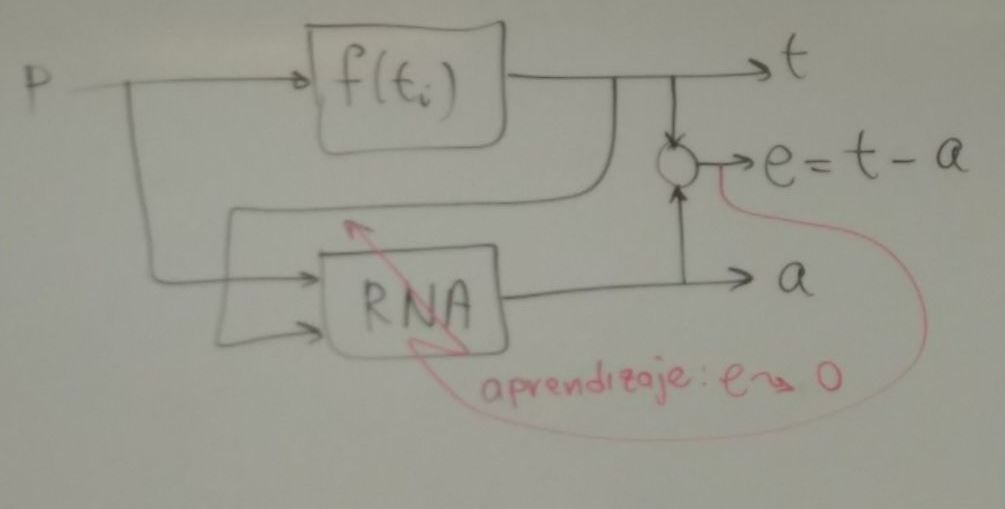
\includegraphics[scale=0.6]{modeloGeneralRn}
\end{figure}

\end{document}
